\section{Analysis and Results}
\label{sec:result-and-analysis}
This section compares the corrected \textit{CodeShovel} oracle with the original \textit{CodeShovel} and \textit{CodeTracker} oracles. It then evaluates the accuracy and runtime efficiency of all method change history generation tools using the corrected \textit{CodeShovel} and the newly developed \textit{HistoryFinder} oracles. In particular, it answers the following three research questions.
\begin{itemize}
    \item \textbf{RQ1}: To what extent does the corrected \textit{CodeShovel} oracle differ from the original oracles?
    \item \textbf{RQ2}: Which history generation tool exhibits the highest accuracy when evaluated with the two new oracles?
    \item \textbf{RQ3}: Which history generation tool exhibits the best runtime performance?
\end{itemize}
\subsection{RQ1: Difference with the corrected CodeShovel oracle}

After correcting the 200 method histories in both the \textit{CodeShovel} and \textit{CodeTracker} oracles, the new systematically constructed oracle—\emph{the corrected CodeShovel oracle}—was compared with the original \textit{CodeShovel} and \textit{CodeTracker} oracles, revealing significant updates. Table~\ref{tab:oracle-update-statistics} provides a detailed breakdown of the changes. It shows how many methods were \emph{changed}, commits were \emph{added}, and \emph{removed}. A method is considered \emph{changed} if the new oracle has a different set of commits than the original. A commit is considered \emph{added} if it was not present in the original oracles, and \emph{removed} if it was inaccurately included. For example, the last column shows that the \textit{CodeTracker} oracle has fewer inaccurate commits (67) than the original \textit{CodeShovel} oracle. In contrast, it missed many commits that should have been recorded as change commits for those 200 methods, as shown in the \emph{\# Added} column.

Compared to the original \textit{CodeShovel} oracle, the histories of 40 methods were \emph{modified}, with 59 commits \emph{added} and 186 \emph{removed}. These changes exclude annotations, JavaDocs, and formatting—omitted by the original \textit{CodeShovel} and \textit{CodeTracker} oracles, though \textit{CodeTracker} did include annotations. When these types of changes were included, 142 method histories were affected, and 429 commits were \emph{added}. Significant changes were also observed when compared with the \textit{CodeTracker} oracle. These changes suggest that the previous evaluations of method tracing tools (e.g., \textit{CodeShovel} and \textit{CodeTracker}) may not reflect the true precision and recall of these tools in tracing a method's change history.


\begin{table}[t]
\centering
\caption{Comparison between the corrected and original oracles. As the corrected oracle includes changes related to annotations, JavaDocs, and formatting, the differences are shown both including (\emph{Incl.}) and excluding (\emph{Excl.}) those changes.}
\label{tab:oracle-update-statistics}
% \resizebox{\linewidth}{!}{%
\begin{tabular}{lrrrrr}
\toprule
\multirow{3}{*}{\textbf{Oracle}}

& \multicolumn{2}{c}{\textbf{\# Methods}} & \multicolumn{3}{c}{\textbf{\# Commits}}\\
\cmidrule(lr){2-3} \cmidrule(lr){4-6}

& \multicolumn{2}{c}{\textbf{\# Changed}} & \multicolumn{2}{c}{\textbf{\# Added}} & \textbf{\# Removed} \\
 & \textbf{Incl.} & \textbf{Excl.} & \textbf{Incl.} & \textbf{Excl.} & \\
\cmidrule(lr){1-1} \cmidrule(lr){2-3} \cmidrule(lr){4-6}
CodeShovel & 142 & 40 &  429 & 59 & 186 \\
CodeTracker & 133 & 43 &  445 & 134 & 67 \\
\bottomrule
\end{tabular}
% }
\end{table}



To illustrate inaccuracies in both the \textit{CodeShovel} and \textit{CodeTracker} oracles, several cases are highlighted. One representative example is the \texttt{fireErrors} method from the \texttt{checkstyle} project. Both the \textit{CodeShovel}\footnote{\href{https://github.com/SQMLab/HistoryFinder/blob/main/oracle/codeshovel-oracle/checkstyle-Checker-fireErrors.json}{https://github.com/SQMLab/HistoryFinder/blob/main/oracle/codeshovel-oracle/checkstyle-Checker-fireErrors.json}} and \textit{CodeTracker}\footnote{\href{https://github.com/SQMLab/HistoryFinder/blob/main/oracle/codetracker-oracle/checkstyle-Checker-fireErrors.json}{https://github.com/SQMLab/HistoryFinder/blob/main/oracle/codetracker-oracle/checkstyle-Checker-fireErrors.json}} oracles record this method’s history beginning from commit \texttt{119fd4}, where the method resided in \path{src/main/java/com/puppycrawl/tools/checkstyle/Checker.java}. However, both oracles incorrectly identified commit \texttt{0e3fe} as the method’s introduction, whereas it was actually introduced earlier in commit \texttt{0fd69} (the method name was \texttt{displayErrors} and was later renamed to \texttt{fireErrors}). This error was recently corrected in the \textit{CodeTracker} oracle; however, the evaluation was conducted using the original published version, where the issue was present.

In another case (\texttt{createPattern method}) in the \textit{CodeShovel} oracle\footnote{\href{https://github.com/checkstyle/checkstyle/compare/d2551035044a845fd1b3e345f2470875a43a8991...f2c6263e151e8a7300755b36fbb41511c0a0cca1\#diff-1b66e778c19cac5ac2beaec4d6a74c8c37a5fd83d39db4bef8c1b60b9ec68c0e}{https://github.com/checkstyle/checkstyle/compare/d2551035044a845fd1b3e345f2470875a43a8991...\allowbreak f2c6263e151e8a7300755b36fbb41511c0a0cca1\#diff-1b66e778c19cac5ac2beaec4d6a74c8c37a5fd83d39db4bef\allowbreak 8c1b60b9ec68c0e last accessed: July 3, 2026}}, while saving the history of an overloaded method, the history failed to stop at the point where the overloaded method was introduced and inaccurately switched to tracing the original of the overloaded method, resulting in incorrect method changes in the oracle. Another challenge arises when handling merge commits. While the \textit{CodeShovel} oracle completely ignored changes that occurred in merge commits, the \textit{CodeTracker} oracle occasionally added incorrect method changes. An example of this issue occurs in the \texttt{runChild} method of the \texttt{junit4} project. Although the diff\footnote{\href{https://github.com/junit-team/junit4/compare/8ff0b44e3fb0c1c56a1dc6290c3b6828a5a8f9bf...bed58a573c373d57d64fa369f58b2a8f0dbee3d7\#diff-cd3bb9170f8d6404c5dc5bb66f7b647435854d48fe357e0bd998e3011a575929}{https://github.com/junit-team/junit4/compare/8ff0b44e3fb0c1c56a1dc6290c3b6828a5a8f9bf...\allowbreak bed58a573c373d57d64fa369f58b2a8f0dbee3d7\#diff-cd3bb9170f8d6404c5dc5bb66f7b647435854d48fe357e0bd\allowbreak998e3011a575929 last accessed: July 3, 2026}} appears to show a method change, it is incorrect—the commit has two parents,\footnote{\href{https://github.com/junit-team/junit4/blob/a49240ade1974b948b20cf2c45d9129f04122735/src/main/java/org/junit/runners/BlockJUnit4ClassRunner.java\#L64}{https://github.com/junit-team/junit4/blob/a49240ade1974b948b20cf2c45d9129f04122735\allowbreak/src/main/java/org/junit/runners/BlockJUnit4ClassRunner.java\#L64 last accessed: July 3, 2026}} and the comparison was made against the wrong parent.\footnote{\href{https://github.com/junit-team/junit4/blob/708ed373c02b467422890d5163fff46d1f32ab01/src/main/java/org/junit/runners/BlockJUnit4ClassRunner.java\#L66}{https://github.com/junit-team/junit4/blob/708ed373c02b467422890d5163fff46d1f32ab01\allowbreak/src/main/java/org/junit/runners/BlockJUnit4ClassRunner.java\#L66 last accessed: July 3, 2026}} In reality, the code was introduced from the other branch\footnote{\href{https://github.com/junit-team/junit4/blob/9d8bb069f68e2194db742981972c8930381b62c2/src/main/java/org/junit/runners/BlockJUnit4ClassRunner.java\#L65}{https://github.com/junit-team/junit4/blob/9d8bb069f68e2194db742981972c8930381b62c2\allowbreak/src/main/java/org/junit/runners/BlockJUnit4ClassRunner.java\#L65 last accessed: July 3, 2026}} without any modification.

\begin{framed}
\noindent\textbf{\underline{RQ1 summary}:}
Both the \textit{CodeShovel} and \textit{CodeTracker} oracles contain inaccuracies in their constructed method histories. The updated, more accurate oracle can serve as a valuable resource for effectively evaluating both existing and future method-level change history generation tools.
\end{framed}

\subsection{RQ2: Accuracy of the change history generation tools}
\label{sec:rq2-accuracy}
The accuracy of six method change history generation tools, including the newly proposed \textit{HistoryFinder}, is evaluated next. This evaluation uses the corrected \textit{CodeShovel} oracle (200 methods) and the new \textit{HistoryFinder} oracle (another 200 methods). The \textit{CodeShovel} oracle is divided into two parts: \textit{CodeShovel Training} and \textit{Testing} oracles. This distinction is important, as both the \textit{CodeShovel} and \textit{HistoryFinder} algorithms were trained and tuned using the training portion of the \textit{CodeShovel} oracle. The three research-based tools were run as Java libraries to extract method histories and compute accuracy metrics. For Git-based tools, the command \texttt{git log <commit> --no-merges -L :<funcname>:<file>} was used to generate method histories for \textit{GitFuncName}, which tracks changes by function name, and \texttt{git log <commit> --no-merges\allowbreak{} -L <start>,\allowbreak{}<end>:<file>} was used for \textit{GitLineRange}, which tracks changes by line range. In contrast, for \textit{IntelliJ}, IntelliJ IDEA 2024.3 Community Edition was used to manually generate method histories (\texttt{Right-click} $\rightarrow$ \texttt{Git} $\rightarrow$ \texttt{Show History for Selection}), as no automated approach exists for running IntelliJ's method tracking feature.

Precision, recall, and F1 score were calculated for all the tools against the three oracles. Since tools differ in the types of changes they detect (e.g., \textit{CodeShovel} ignores annotations, \textit{CodeTracker} ignores formatting), the expected commit sets were tailored to match each tool’s capabilities, ensuring a fair and meaningful comparison. The tools' accuracy is evaluated at two granularities: \emph{commit-level} and \emph{method-level}. At the \emph{commit-level}, precision, recall, and F1 scores are computed by aggregating true positives (TP), false positives (FP), and false negatives (FN) across each oracle, based on the total expected commits. At the \emph{method-level}, metrics are computed per method and averaged across each oracle.

\begin{table*}[t]
\centering
\caption{Precision, recall, and F1 score for method history tracking tools across three oracles.
\textbf{TP} (True Positives) indicates correctly identified change commits;
\textbf{FP} (False Positives) refers to incorrectly included commits;
\textbf{FN} (False Negatives) denotes missed commits that should have been identified. \textbf{Bolded values indicate the best performance in each metric within an oracle.}}
\label{tab:hf-method-tracking-score}
\resizebox{\textwidth}{!}{%
% \small
% \setlength{\tabcolsep}{3pt}
\begin{tabular}{llrrrrrrrrr}
\toprule
\multirow{2}{*}{\textbf{Oracle}} & \multirow{2}{*}{\textbf{Tool}} & \multicolumn{6}{c}{\textbf{\emph{Commit-Level}}} & \multicolumn{3}{c}{\textbf{\emph{Method-Level}}} \\
\cmidrule(lr){3-8} \cmidrule(lr){9-11}
 &  & \textbf{TP} & \textbf{FP} & \textbf{FN} & \textbf{Precision} & \textbf{Recall} & \textbf{F1} & \textbf{Precision} & \textbf{Recall} & \textbf{F1} \\

\cmidrule(lr){1-1} \cmidrule(lr){2-2} \cmidrule(lr){3-5}  \cmidrule(lr){6-8} \cmidrule(lr){9-11}

\multirow{6}{*}{CodeShovel Training}
    & CodeShovel & 2813 & 158 & 28 & 94.68 & \textbf{99.01} & 96.80 & 94.79 & \textbf{99.31} & 95.86 \\
    & CodeTracker & 2804 & 32 & 76 & 98.87 & 97.36 & 98.11 & 98.99 & 96.98 & 97.52 \\
    & HistoryFinder & 3047 & 6 & 67 & \textbf{99.80} & 97.85 & \textbf{98.82} & \textbf{99.68} & 98.15 & \textbf{98.53} \\
    & IntelliJ & 2146 & 402 & 919 & 84.22 & 70.02 & 76.47 & 85.16 & 75.08 & 73.40 \\
    & GitLineRange & 2197 & 1135 & 787 & 65.94 & 73.63 & 69.57 & 77.94 & 76.32 & 68.29 \\
    & GitFuncName & 1749 & 1166 & 1261 & 60.00 & 58.11 & 59.04 & 72.93 & 62.03 & 54.88 \\
\cmidrule(lr){1-1} \cmidrule(lr){2-2} \cmidrule(lr){3-5}  \cmidrule(lr){6-8} \cmidrule(lr){9-11}
\multirow{6}{*}{CodeShovel Testing}
    & CodeShovel & 812 & 25 & 38 & 97.01 & 95.53 & 96.27 & 97.40 & 95.70 & 95.54 \\
    & CodeTracker & 811 & 35 & 63 & 95.86 & 92.79 & 94.30 & 97.59 & 94.36 & 94.76 \\
    & HistoryFinder & 938 & 10 & 7 & \textbf{98.95} & \textbf{99.26} & \textbf{99.10} & \textbf{99.15} & \textbf{99.24} & \textbf{99.15} \\
    & IntelliJ & 685 & 239 & 249 & 74.13 & 73.34 & 73.74 & 85.14 & 72.58 & 73.78 \\
    & GitLineRange & 609 & 288 & 279 & 67.89 & 68.58 & 68.24 & 87.48 & 70.02 & 72.31 \\
    & GitFuncName & 579 & 393 & 331 & 59.57 & 63.63 & 61.53 & 77.85 & 65.34 & 65.35 \\
\cmidrule(lr){1-1} \cmidrule(lr){2-2} \cmidrule(lr){3-5}  \cmidrule(lr){6-8} \cmidrule(lr){9-11}
\multirow{6}{*}{HistoryFinder}
    & CodeShovel & 2095 & 147 & 394 & 93.44 & 84.17 & 88.56 & 95.68 & 86.45 & 85.82 \\
    & CodeTracker & 2354 & 88 & 168 & \textbf{96.40} & 93.34 & 94.84 & 94.43 & 91.24 & 94.14 \\
    & HistoryFinder & 2835 & 106 & 48 & \textbf{96.40} & \textbf{98.34} & \textbf{97.36} & \textbf{96.49} & \textbf{96.81} & \textbf{97.00} \\
    & IntelliJ & 2185 & 1530 & 637 & 58.82 & 77.43 & 66.85 & 75.99 & 81.38 & 75.80 \\
    & GitLineRange & 2032 & 2112 & 616 & 49.03 & 76.74 & 59.84 & 77.64 & 82.98 & 75.50 \\
    & GitFuncName & 1858 & 2638 & 835 & 41.33 & 68.99 & 51.69 & 65.08 & 72.67 & 59.50 \\
\bottomrule
\end{tabular}
}
\end{table*}

Table~\ref{tab:hf-method-tracking-score} shows that all research-based tools—\textit{CodeShovel}, \textit{CodeTracker}, and \textit{HistoryFinder}—significantly outperform \textit{IntelliJ} and \texttt{Git-based} tools. Overall, \textit{HistoryFinder} achieves the highest F1 score. In terms of precision, \textit{HistoryFinder} and \textit{CodeTracker} slightly outperform \textit{CodeShovel}. For recall, \textit{CodeShovel} performs best on its own training oracle; however, on the other two oracles, \textit{HistoryFinder} achieves the highest recall. \textit{CodeShovel’s} notably lower recall on the \textit{HistoryFinder} oracle is primarily due to its failure to generate the complete history for several methods. For example, it was unable to produce complete histories for all 10 methods from the Cassandra project. Additionally, it failed entirely for two methods in the Fastjson project due to \texttt{JavaParser} errors that prevented successful file parsing. Overall, across all three oracles, \textit{HistoryFinder} demonstrates the most consistent and superior performance. Results at the \emph{method-level} scores closely correlate with \emph{commit-level} scores, with minor variations. For instance, \textit{CodeShovel's} precision against the \textit{HistoryFinder} oracle is approximately 2\% higher at the \emph{method-level} compared to the \emph{commit-level}.
The Wilcoxon rank-sum test~\cite{wilcoxon_individual_1945} also shows that the observed accuracy gain with \textit{HistoryFinder} is statistically significant ($P \le 0.05$).

\begin{framed}
\noindent\textbf{\underline{RQ2 summary}:}
The \textit{HistoryFinder} algorithm consistently achieves the highest precision and F1 score in change history detection. Between \textit{CodeShovel} and \textit{CodeTracker}, performance varies depending on the scenario. Notably, \textit{CodeShovel's} recall drops significantly on the entirely new oracle of 200 methods, mainly because it fails to generate the full or any history for a subset of methods. Given these findings, researchers or practitioners who prioritize accuracy should consider \textit{HistoryFinder} the most reliable option.
\end{framed}

\subsection{RQ3: Runtime performance of the change history generation tools}
\label{sec:rq3-runtime}

The tools were executed in a controlled environment on a machine equipped with \emph{32GB of RAM, an Intel(R) Core(TM) i7-8700 CPU @ 3.20GHz with 12 cores, running Ubuntu 22.04 LTS and Java 21 x86}. Execution time for \textit{IntelliJ} was not recorded since method histories were generated manually from \texttt{IntelliJ IDEA}, making it infeasible to measure the time. Prior to recording execution time, all repositories were cloned to a local persistent storage. Initially, the JAR dependencies of the research-based tools were integrated. However, caching of parsed Java files across multiple method history runs—particularly in \textit{CodeShovel}—was observed to significantly reduce the runtime. While this optimization benefits batch processing, it does not yield deterministic or representative runtimes for tracing individual methods. To ensure a fair comparison, each tool was instead executed independently for each method history using the \texttt{java -jar} command. This approach ensured that each method's history was processed in isolation within a fresh environment, by launching a separate \texttt{JAR} process for each run and terminating it upon completion. Please note that due to the deterministic nature of the evaluated tools, the difference in execution times in multiple runs for a given tool is negligible.

\begin{figure*}[t]
  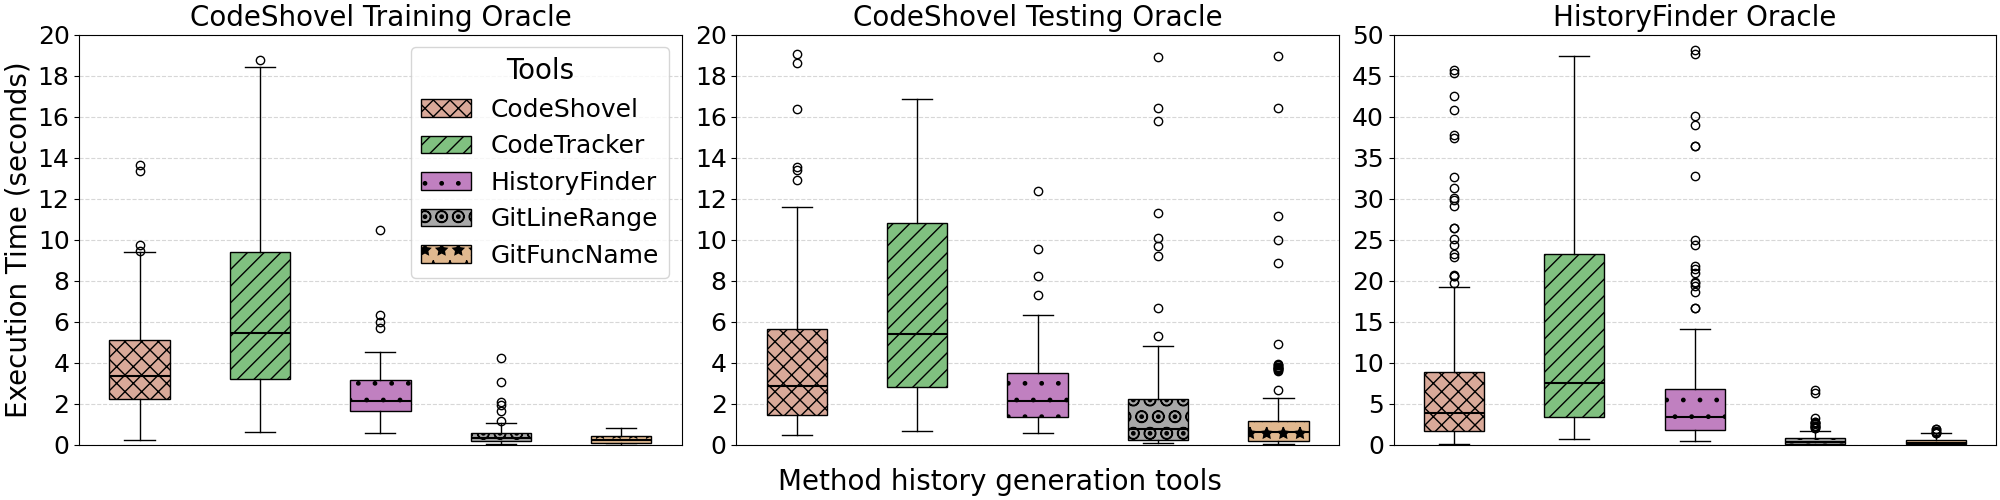
\includegraphics[width=\linewidth]{figure/execution-time-box-plot.png}
\caption{Comparison of execution times across three oracles for five tools. To enhance readability, the y-axis is limited to 20 seconds for the first two subplots (\textit{CodeShovel} oracles) and 50 seconds for the third subplot (\textit{HistoryFinder} oracle).}
% \Description{Comparison of execution times across three oracles for five tools. To enhance readability, the y-axis is limited to 20 seconds for the first two subplots (\textit{CodeShovel} oracles) and 50 seconds for the third subplot (\textit{HistoryFinder} oracle).}
\label{fig:execution-time-box-plot}
\end{figure*}



\begin{table}[ht]

\centering
\caption{Execution times (in seconds) for the five tools. \textit{IntelliJ} is excluded because of the need for manual execution.}
% \Description{Mean, median, minimum, and maximum execution times (in seconds) for five tools.
% \textbf{Bold} values indicate the best (lowest) execution time for both research-based and \texttt{Git}-based tools. \textit{IntelliJ} is excluded because method histories for this tool were generated manually using the \texttt{IDEA} interface.}
% \resizebox{\linewidth}{!}{%
\begin{tabular}{llrrrr}
\toprule
\textbf{Oracle} & \textbf{Tool} & \textbf{Mean} & \textbf{Median} & \textbf{Min} & \textbf{Max} \\ \midrule
\multirow{5}{*}{\makecell{CodeShovel\\Training}}
    & CodeShovel & 3.93 & 3.38 & \textbf{0.22} & 13.63 \\
    & CodeTracker & 8.71 & 5.45 & 0.64 & 76.80 \\
    & HistoryFinder & \textbf{2.51} & \textbf{2.15} & 0.59 & \textbf{10.48} \\
    \cmidrule(lr){2-2} \cmidrule(lr){3-6}
    & GitLineRange & 0.50 & 0.35 & 0.07 & 4.23 \\
    & GitFuncName & \textbf{0.26} & \textbf{0.24} & \textbf{0.02} & \textbf{0.83} \\
\cmidrule(lr){1-1} \cmidrule(lr){2-2} \cmidrule(lr){3-6}
\multirow{5}{*}{\makecell{CodeShovel\\Testing}}
    & CodeShovel & 4.55 & 2.86 & \textbf{0.49} & 26.08 \\
    & CodeTracker & 9.29 & 5.42 & 0.68 & 63.34 \\
    & HistoryFinder & \textbf{2.85} & \textbf{2.15} & 0.57 & \textbf{20.78} \\
    \cmidrule(lr){2-2} \cmidrule(lr){3-6}
    & GitLineRange & 2.13 & 0.80 & 0.11 & \textbf{18.93} \\
    & GitFuncName & \textbf{1.57} & \textbf{0.61} & \textbf{0.07} & 18.94 \\
\cmidrule(lr){1-1} \cmidrule(lr){2-2} \cmidrule(lr){3-6}
\multirow{5}{*}{HistoryFinder}
    & CodeShovel & 7.74 & 3.88 & \textbf{0.15} & \textbf{74.49} \\
    & CodeTracker & 30.41 & 7.56 & 0.76 & 693.66 \\
    & HistoryFinder & \textbf{7.32} & \textbf{3.47} & 0.49 & 106.64 \\
    \cmidrule(lr){2-2} \cmidrule(lr){3-6}
    & GitLineRange & 0.69 & 0.38 & 0.04 & 6.66 \\
    & GitFuncName & \textbf{0.41} & \textbf{0.21} & \textbf{0.03} & \textbf{1.96} \\
\bottomrule

\end{tabular}
% }
\label{tab:execution-time-statistic}
\end{table}

Figure~\ref{fig:execution-time-box-plot} shows the distribution of execution times for all five tools across the three oracles, while Table~\ref{tab:execution-time-statistic} presents the mean, median, minimum, and maximum execution times. Excluding outliers, \textit{HistoryFinder} demonstrates the lowest execution times among the three research-based tools. In general, \textit{CodeTracker} is the slowest in constructing method change history. Across all tools and oracles, the minimum execution time consistently remained below one second. However, for the research-based tools, although the mean and median execution times are slightly higher in the \emph{HistoryFinder} oracle compared to the \emph{CodeShovel} oracle, the difference in maximum execution time between these two oracles is unexpectedly large.

To understand the factors contributing to the increased runtime in the \textit{HistoryFinder} oracles, cases with unusually high execution times were manually examined. Prolonged runtimes were often linked to a high frequency of changes in the file containing the target method, regardless of whether the method itself was modified. In such cases, parsing a high number of Java files using the \texttt{JavaParser} was particularly time-consuming. Profiling of the tools revealed that, for methods with high execution times, over 80\% of the total runtime was typically spent on parsing alone, thereby significantly increasing the computational overhead. Repositories like Kafka, Cassandra, Jenkins, and Pulsar frequently exhibited these patterns, and these types of projects are more prevalent in the \textit{HistoryFinder} oracle compared to the \textit{CodeShovel} oracle.

\textit{CodeTracker} exhibited significantly high execution times when a method or its enclosing file was moved in a commit that also modified many other files—a pattern observed in repositories such as Netty and ShardingSphere. In contrast, \textit{CodeShovel}'s maximum execution time on the \textit{HistoryFinder} oracle was much lower than that of \textit{CodeTracker} and \textit{HistoryFinder}. However, this lower runtime is primarily due to \textit{CodeShovel} failing to generate complete histories for many complex methods with extensive change histories—cases where both \textit{CodeTracker} and \textit{HistoryFinder} succeeded.


The \texttt{Git-based} tools, in contrast, did not exhibit high execution times in the \textit{HistoryFinder} oracle. Their maximum execution times were also significantly lower than those of the research-based tools. This lower runtime is primarily due to two factors: (i) \texttt{Git-based} tools operate using \texttt{git log} without relying on language-specific parsers. Instead, they track line-level changes, making their execution comparatively lightweight; and (ii) similar to \textit{CodeShovel}, these tools often failed to recover the complete change histories of complex methods. As a result, their efficiency comes at the cost of significantly lower precision and recall compared to their research-based counterparts, as also reflected in Table~\ref{tab:hf-method-tracking-score}.

\begin{framed}
\noindent\textbf{\underline{RQ3 summary}:}
\texttt{Git-based} tools exhibit the lowest execution times, but this efficiency comes at the cost of significantly reduced accuracy. Among research-based tools, \textit{HistoryFinder} strikes the best balance of speed and accuracy, while \textit{CodeTracker}, the second most accurate, shows the highest and most variable runtimes. Overall, \textit{HistoryFinder} is the most reliable choice for those prioritizing accuracy and speed.
\end{framed}
